\documentclass{article}
\usepackage[T1]{fontenc}
\usepackage{lmodern}
\usepackage{graphicx}
\usepackage{amsmath,amssymb}
\usepackage[a4paper,margin=2cm]{geometry}
\usepackage[absolute,overlay]{textpos}
\setlength{\TPHorizModule}{1mm}
\setlength{\TPVertModule}{1mm}
\usepackage[indonesian]{babel}
\usepackage{hyperref}
\setlength{\emergencystretch}{2em}
% unit: Halaman 36

\begin{document}

% === Halaman 36 (llm) ===

\section*{Kunci-kunci lemah DES}

\vspace{130.68mm}

\begin{itemize}
    \item \textbf{Kunci lemah DES} adalah kunci K sedemikian sehingga $E_K(E_K(x)) = x$ untuk semua plainteks x, yang artinya enkripsi dan dekripsi menjadi sama.
    \begin{itemize}
        \item Kunci lemah ini menghasilkan pembangkitan kunci putaran yang sama pada semua putaran.
    \end{itemize}
\end{itemize}

\begin{itemize}
    \item DES memiliki 4 kunci lemah (masing-masing panjangnya 56 bit), dinyatakan dalam kode heksadesimal sbb:
    \begin{align*}
        &0000000000000000 \\
        &0000000FFFFFFFF \\
        &FFFFFFF00000000 \\
        &FFFFFFFFFFFFFFFF
    \end{align*}
    \vspace{10mm}
    \item Kunci lemah seharusnya dihindari.
\end{itemize}

% deskripsi: Ilustrasi dua buah kunci berwarna kuning yang terikat pada satu gantungan kunci
% bbox normalisasi: [0.6500, 0.4700, 0.8550, 0.9100]
\begin{textblock*}{43.05mm}(136.50mm,139.59mm)
\noindent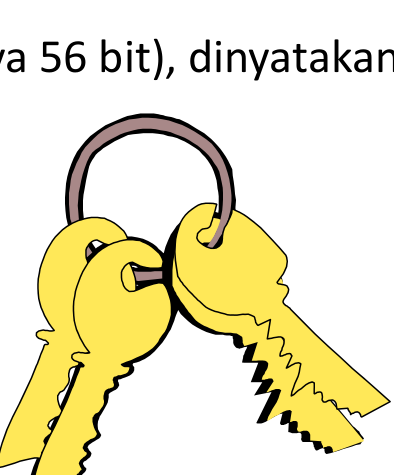
\includegraphics[width=43.05mm,height=130.68mm]{../../images/llm/page_036_img_01.png}%
\end{textblock*}

\end{document}
